\documentclass[8pt]{article}
\usepackage[a4paper,landscape,margin=1in]{geometry}
\usepackage{cmbright}

\usepackage{amsmath}
\usepackage{nicefrac}
\usepackage{siunitx}

\usepackage{array}
\usepackage{booktabs}
\usepackage{longtable}

\usepackage{xcolor}
\definecolor{urlblue}{HTML}{0000ee}
\usepackage{hyperref}
\hypersetup{%
colorlinks = true,%
urlcolor   = urlblue,%
}

\usepackage{tcolorbox}
\usepackage{varwidth}

\setlength\parindent{0pt}
\pagenumbering{gobble}

\begin{document}
\begin{figure}[!ht]
% MF group logo
\begin{minipage}[b][2.5cm][c]{.72\textwidth}
\href{http://foroozandeh.chem.ox.ac.uk/home}%
{\includegraphics[scale=1.8]{/home/simon/Documents/DPhil/projects/spectral_estimation/NMR-EsPy/nmrespy/images/mf_logo.png}}
\end{minipage}
% NMR-EsPy logo
\begin{minipage}[b][2.5cm][c]{.27\textwidth}
\href{https://foroozandehgroup.github.io/NMR-EsPy}%
{
\includegraphics[scale=0.5]{/home/simon/Documents/DPhil/projects/spectral_estimation/NMR-EsPy/nmrespy/images/nmrespy_full.png}}
\end{minipage}
\end{figure}

\texttt{10:20:29\\24-09-2021}

% user provided description
\subsection*{Description}
Gramicidin \textsuperscript{{1}}H data, region: 3.05 - 2.7Hz. MPM result.

% experiment parameters
\subsection*{Experiment Information}
\hspace{-6pt}
\begin{longtable}[l]{c c}
\toprule
Parameter & F1
\\\midrule
Transmitter frequency (MHz) & 699.85349925\\
Sweep width (Hz) & 318.74730253669054\\
Sweep width (ppm) & 0.455448608713505\\
Transmitter offset (Hz) & 2012.191011955847\\
Transmitter offset (ppm) & 2.8751603215704673\\
\bottomrule
\end{longtable}

% estimation result
\subsection*{Result}
\begin{longtable}[l]{c c c c c c c c}
\toprule
$m$ & $a_m$ & $\phi_m\ (\text{rad})$ & $f_m\ (\text{Hz})$ & $f_m\ (\text{ppm})$ & $\eta_m\ (\text{s}^{-1})$ & $\int$ & $\nicefrac{\int}{\left\lVert\int\right\rVert}$
\\\midrule
1 & 17.238 & 3.0586 & \num{1.8996e+3} & 2.7143 & 53.305 & \num{1.7027e+4} & \num{4.1554e-2}\\
2 & 0.92919 & \num{-8.3203e-2} & \num{1.9136e+3} & 2.7343 & 8.7117 & 918.03 & \num{2.2404e-3}\\
3 & 30.711 & 0.63392 & \num{1.9235e+3} & 2.7485 & 53.599 & \num{2.5045e+4} & \num{6.112e-2}\\
4 & 11.404 & 0.4649 & \num{1.9297e+3} & 2.7573 & 12.42 & \num{1.1152e+4} & \num{2.7215e-2}\\
5 & 47.654 & \num{8.9546e-2} & \num{1.9367e+3} & 2.7673 & 16.772 & \num{4.7061e+4} & 0.11485\\
6 & 64.94 & 0.38629 & \num{1.9425e+3} & 2.7755 & 15.431 & \num{6.119e+4} & 0.14933\\
7 & 86.178 & -0.34625 & \num{1.9503e+3} & 2.7868 & 16.656 & \num{8.075e+4} & 0.19706\\
8 & 76.052 & -0.11197 & \num{1.9562e+3} & 2.7952 & 17.392 & \num{7.493e+4} & 0.18286\\
9 & 26.173 & -0.9512 & \num{1.9637e+3} & 2.8058 & 15.055 & \num{2.8541e+4} & \num{6.9651e-2}\\
10 & 39.939 & -1.9827 & \num{1.9705e+3} & 2.8156 & 20.298 & \num{4.2125e+4} & 0.1028\\
11 & 62.688 & -0.53925 & \num{1.9748e+3} & 2.8217 & 20.491 & \num{5.8391e+4} & 0.1425\\
12 & 135.36 & -0.29092 & \num{1.9818e+3} & 2.8317 & 22.464 & \num{1.2856e+5} & 0.31375\\
13 & 130.21 & 0.42154 & \num{1.987e+3} & 2.8392 & 19.999 & \num{1.2036e+5} & 0.29374\\
14 & 97.847 & -0.38066 & \num{1.9951e+3} & 2.8508 & 17.913 & \num{9.1181e+4} & 0.22252\\
15 & 62.582 & -0.37161 & \num{2.0006e+3} & 2.8586 & 17.071 & \num{5.8505e+4} & 0.14278\\
16 & 100.72 & \num{7.4836e-2} & \num{2.003e+3} & 2.862 & 12.588 & \num{9.9587e+4} & 0.24303\\
17 & 140.05 & 0.21751 & \num{2.0074e+3} & 2.8683 & 27.53 & \num{1.3558e+5} & 0.33088\\
18 & 125.92 & 0.43065 & \num{2.013e+3} & 2.8763 & 13.082 & \num{1.2132e+5} & 0.29608\\
19 & 77.879 & 0.60859 & \num{2.0156e+3} & 2.88 & 10.234 & \num{8.2121e+4} & 0.20041\\
20 & 97.117 & 0.13603 & \num{2.026e+3} & 2.8949 & 12.21 & \num{9.54e+4} & 0.23281\\
21 & 11.991 & -1.2834 & \num{2.0332e+3} & 2.9051 & 19.903 & \num{1.2923e+4} & \num{3.1536e-2}\\
22 & 1.9739 & -1.2324 & \num{2.0404e+3} & 2.9155 & 12.186 & \num{2.4001e+3} & \num{5.8572e-3}\\
23 & 3.1642 & -0.30394 & \num{2.0516e+3} & 2.9314 & 9.4184 & \num{3.0533e+3} & \num{7.4514e-3}\\
24 & 5.6327 & -0.36151 & \num{2.0574e+3} & 2.9398 & 11.317 & \num{5.4213e+3} & \num{1.323e-2}\\
25 & 3.5387 & -0.6869 & \num{2.0646e+3} & 2.9501 & 9.1528 & \num{3.9185e+3} & \num{9.5628e-3}\\
26 & 22.636 & -0.15809 & \num{2.0704e+3} & 2.9583 & 19.74 & \num{2.2164e+4} & \num{5.409e-2}\\
27 & 123.34 & 0.27845 & \num{2.0752e+3} & 2.9652 & 15.103 & \num{1.1757e+5} & 0.28691\\
28 & 110.99 & 0.23924 & \num{2.0809e+3} & 2.9733 & 12.036 & \num{1.069e+5} & 0.26088\\
29 & 71.776 & 0.22344 & \num{2.0881e+3} & 2.9836 & 9.8075 & \num{6.9389e+4} & 0.16934\\
30 & 73.308 & \num{9.7574e-2} & \num{2.0939e+3} & 2.9919 & 12.672 & \num{7.2334e+4} & 0.17652\\
31 & 115.12 & -2.2448 & \num{2.0979e+3} & 2.9976 & 138.23 & \num{7.1711e+4} & 0.175\\
\bottomrule
\end{longtable}

% figure of result
\begin{center}
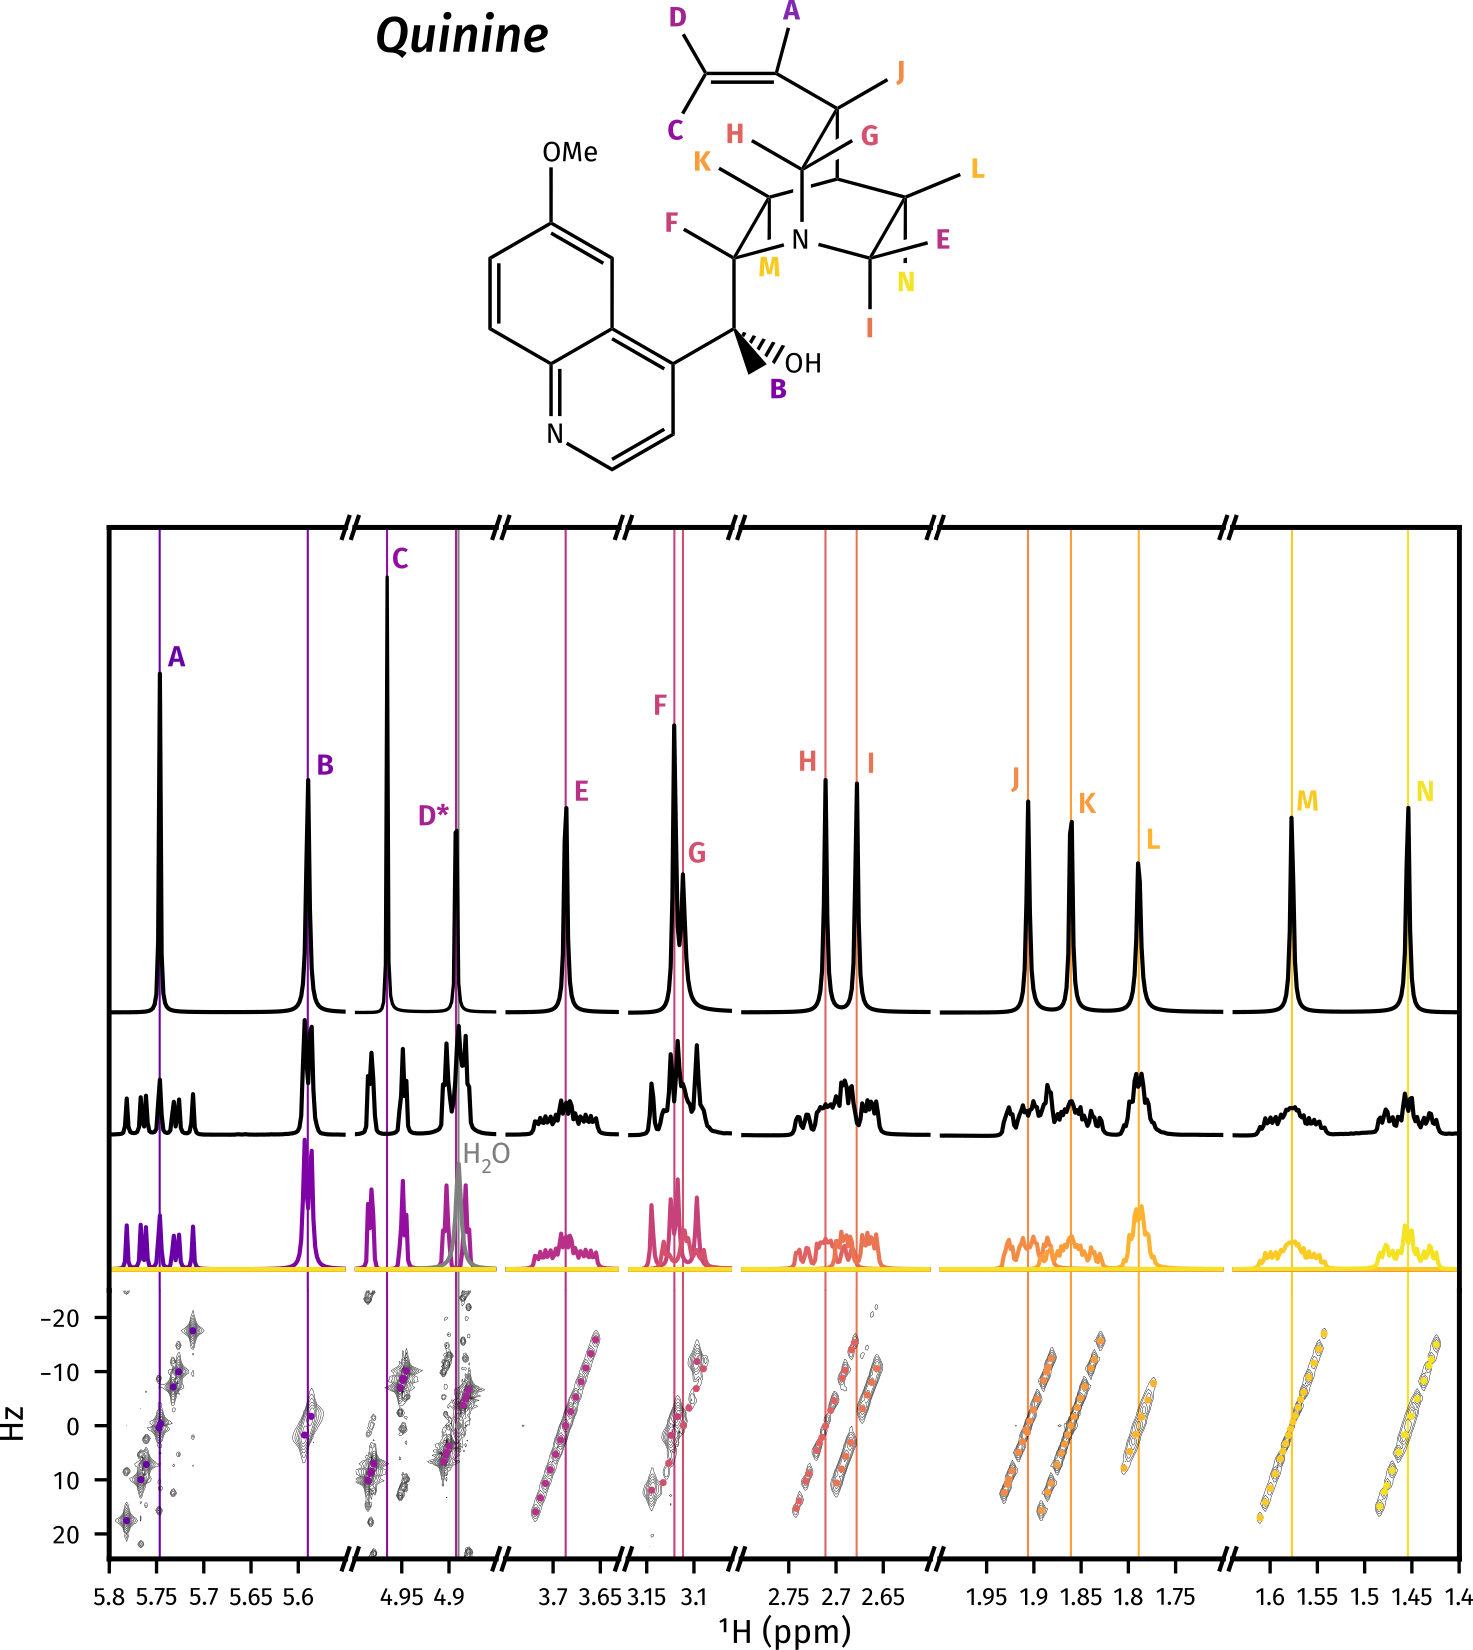
\includegraphics{/tmp/figure.pdf}
\end{center}

% blurb
\small
\begin{tcolorbox}[hbox]
\begin{varwidth}{\textwidth}
Estimation performed using \textsc{NMR-EsPy}.\\
Author: Simon Hulse\\
For more information:\\[5pt]
{\raisebox{-4pt}{\includegraphics[scale=0.029]{/home/simon/Documents/DPhil/projects/spectral_estimation/NMR-EsPy/nmrespy/images/book_icon.png}}}\hspace{1em}\href{https://foroozandehgroup.github.io/NMR-EsPy}{\texttt{https://foroozandehgroup.github.io/NMR-EsPy}}\\[5pt]
{\raisebox{-4pt}{
\includegraphics[scale=0.12]{/home/simon/Documents/DPhil/projects/spectral_estimation/NMR-EsPy/nmrespy/images/github.png}}}\hspace{1em}\href{https://github.com/foroozandehgroup/NMR-EsPy}{\texttt{https://github.com/foroozandehgroup/NMR-EsPy}}\\[5pt]
{\raisebox{-3pt}{\includegraphics[scale=0.015]{/home/simon/Documents/DPhil/projects/spectral_estimation/NMR-EsPy/nmrespy/images/email_icon.png}}}\hspace{1em}\href{mailto:simon.hulse@chem.ox.ac.uk?subject=NMR-EsPy query}{\texttt{simon.hulse@chem.ox.ac.uk}}\\[5pt]
If used in a publication, please cite:\\
\textit{No references yet...}
\end{varwidth}
\end{tcolorbox}

\end{document}
